\documentclass[12pt]{article}
\usepackage[12pt]{moresize}
\usepackage[margin=1in]{geometry}

\usepackage{amsmath}
\usepackage{amssymb}

\usepackage{graphicx}
\usepackage{subcaption}

\usepackage{multirow} %Combining rows in tables
\usepackage{diagbox}  %Table box split in twain

\usepackage{algorithm}
\usepackage{algpseudocode}
\usepackage{alltt}

\usepackage{multicol}

\usepackage{amssymb} %\checkmark symbol

%\usepackage{hyperref}
%\usepackage[latin1]{inputenc}
%\usepackage{listings}
%\usepackage{scrextend}
%\usepackage{changepage} %Adjustwidth

 

\title{ComS 474\\Homework 5}
\author{Sean Gordon}
\date{Nov 12, 2020}

\begin{document}
\maketitle



\noindent 1) $
\begin{pmatrix}
0.5 & 0.2 & 0.9\\
-3 & -40 & 1.5
\end{pmatrix}$\\\\

\noindent 2) $
\begin{pmatrix}
1.6 & -36.5\\
2 & -41.5
\end{pmatrix}$
 and $
\begin{pmatrix}
1.6 & 2\\
-36.5 & -41.5
\end{pmatrix}$\\[.4em]

\noindent 3) There is no product AB because their dimensions are not compatible. \\
\indent \# Cols in A != \# Rows in B\\

\noindent 4) $\begin{pmatrix}
1.6 & -36.5\\
2 & -41.5
\end{pmatrix}$ + 1 = $
\begin{pmatrix}
2.6 & -35.5\\
3 & -40.5
\end{pmatrix}$\\\\

\noindent 5) {\Large $\frac{\delta E}{\delta \hat y}$} = {\Large $\frac{\delta (\hat y - y)^2}{\delta \hat y}$} = $2(\hat y - y)$ = $2(w^Tx - y)$\\\\

\noindent 6) $\hat y = \phi(w^Tx) = (1*5)^2+(0*4)^2+(1*6)^2+(0*1)^2 = 61$\\\\

\noindent 7) {\Large $\frac{\delta E}{\delta x_1}$} = {\Large $\frac{\delta ((w_0x_0)^2 + (w_1x_1)^2 + (w_2x_2)^2 + (w_3x_3)^2 - y)}{\delta x_1}$} = $2w_1^2 = 2(4)^2 = 32$\\[.4em]
\indent {\Large $\frac{\delta E}{\delta w_1}$} = {\Large $\frac{\delta ((w_0x_0)^2 + (w_1x_1)^2 + (w_2x_2)^2 + (w_3x_3)^2 - y)}{\delta w_1}$} = $2x_1^2 = 2(0)^2 = 0$\\\\

\noindent 8) {\Large $\frac{\delta E}{\delta x}$} = $2w_0^2 + 2w_1^2 + 2w_2^2 + 2w_3^2$ = $2(5)^2 + 2(4)^2 + 2(6)^2 + 2(1)^2$ = $156$\\[.4em]
\indent {\Large $\frac{\delta E}{\delta x}$} = $2x_0^2 + 2x_1^2 + 2x_2^2 + 2x_3^2$ = $2(1)^2 + 2(0)^2 + 2(1)^2 + 2(0)^2$ = $4$\\[.4em]



%\begin{figure}[htbp]
%\centerline{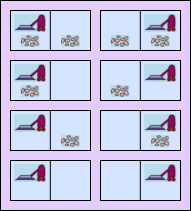
\includegraphics{Pics/ComS472_410.png}}
%\caption{Belief states recheable from initial 8 belief states.}
%\label{Belief states recheable from initial 8 belief states.}
%\end{figure}

\end{document}

















